% 1977 年湖北卷第二题：矩形场地一边靠房屋的墙（斜线段示墙），平行于墙的一边长标 x（按源卷第 3 页布局）
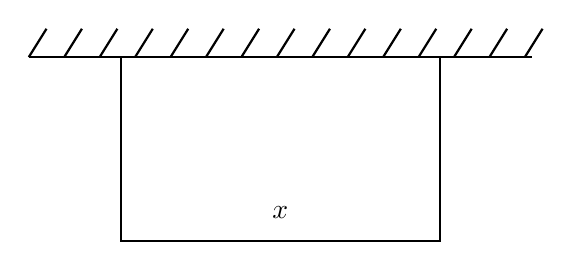
\begin{tikzpicture}[scale=0.9]
  \draw[thick] (0,0) rectangle (4.5,2.6);
  \draw[thick] (-1.3,2.6)--(5.8,2.6);
  \foreach \i in {0,...,14}
    \draw[thick] ({-1.3+0.5*\i},2.6) -- ({-1.05+0.5*\i},3.0);
  \node at (2.25,0.4) {$x$};
\end{tikzpicture}
